\section{Abstract}

This is a literature review document that aims at finding all available deep learning methods and approaches in analyzing different medical images in for various tasks. We will focus on histopathological images but this literature includes all other varieties of images in medical image analysis. 

\clearpage
\section{Search Keywords}

Here are the phrases and the keywords used in the search.

\begin{itemize}
	\item Phrase1: Deep Learning Pathology
	\item Phrase2: Keyword3 Keyword4
\end{itemize}

\clearpage
\section{Search Map}

Here is the search map for this literature review:

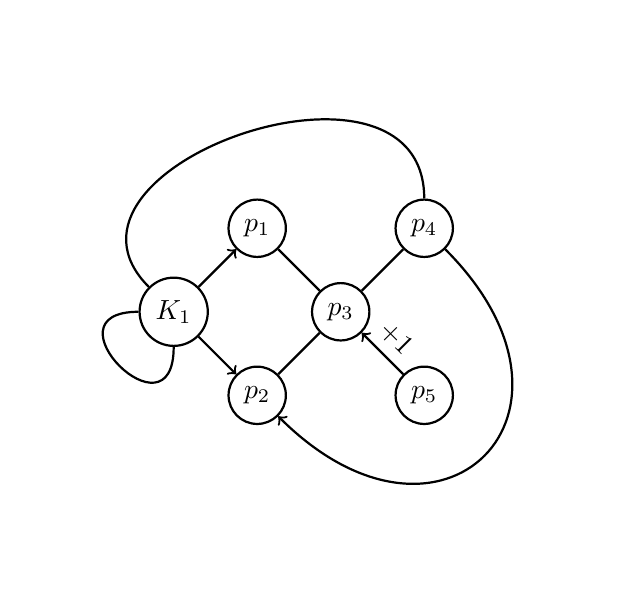
\begin{tikzpicture}[node distance={15mm}, thick, main/.style = {draw, circle}] 
\node[main] (1) {$K_1$}; 
\node[main] (2) [above right of=1] {$p_1$}; 
\node[main] (3) [below right of=1] {$p_2$}; 
\node[main] (4) [above right of=3] {$p_3$}; 
\node[main] (5) [above right of=4] {$p_4$}; 
\node[main] (6) [below right of=4] {$p_5$}; 
\draw[->] (1) -- (2); 
\draw[->] (1) -- (3); 
\draw (1) to [out=135,in=90,looseness=1.5] (5); 
\draw (1) to [out=180,in=270,looseness=5] (1); 
\draw (2) -- (4); 
\draw (3) -- (4); 
\draw (5) -- (4); 
\draw[->] (5) to [out=315, in=315, looseness=2.5] (3); 
\draw[->] (6) -- node[midway, above right, sloped, pos=1] {+1} (4); 
\end{tikzpicture} 